\documentclass[titlepage]{article}
\author{Ryan Kwon, Anthoney Tsou}
\title{An Implementation of Quality Minus Junk}
\date{February 11, 2015}
\usepackage{Sweave}
\begin{document}
\Sconcordance{concordance:paper.tex:paper.Rnw:%
1 2 1 1 0 6 1 5 0 1 4 10 1 1 2 1 0 1 1 1 2 1 0 1 2 1 0 1 2 5 0 1 5 2 0 %
3 1 3 0 1 2 3 1 4 0 1 3 3 1 4 0 1 3 2 1 1 2 1 0 2 1 24 0 1 4 5 0 1 3 8 %
0 1 2 1 3 2 0 1 1 3 0 1 3 8 0 1 2 1 4 3 0 1 2 1 0 1 2 25 0 1 2 2 1 1 3 %
2 0 1 1 18 0 1 5 3 0 1 1 18 0 1 4 2 0 1 1 18 0 1 6 4 0 1 1 19 0 1 2 5 1 %
5 0 1 4 5 0 1 4 5 0 1 4 6 1 7 0 1 6 5 0 1 4 46 1}

\maketitle

\section*{Abstract}
The \textbf{qmj} package produces quality scores for companies based on the work of Asness et. al (2013). It measures the quality of each of the 3000 largest US companies from the Russell 3000 Index based on profitability, growth, safety, and payouts, using the latest available data from Google Finance. The package includes tools to automatically gather relevant financial documents and stock data, allowing users to update their data whenever desired. The package also provides utilities for analyzing the scores of individual companies, various plotting and filtering tools, and generally helps separate the list of companies into ``junk'' stocks, which are expected to underperform relative to the market, and ``quality'' stocks, which are expected to outperform. 

\section*{Introduction}
\textbf{qmj} implements the methodology of the work of \emph{Asness et. al} (2013). Within the paper, Asness uses several financial measures to calculate the relative profitability, growth, safety, and payouts of a company within a given universe, which they use to provide an overall quality score for a company.

This quality score is used as the basis of a portfolio which longs quality companies, which are likely to outperform the market, while ``junk'' companies shorted as they are expected to underperform relative to the market.

\textbf{qmj} provides tools to practically apply their results, coming equipped with pre-compiled recent data in addition to providing tools to automatically update or analyze that information.

\section*{Data}
We demonstrate the use of \textbf{qmj} first based on the already installed data, using a universe comprised of all companies in the Russell 3000 Index as of February 1, 2015.

\begin{Schunk}
\begin{Sinput}
> library(qmj)
> data(companies) 
> data(financials) 
> data(prices) 
> data(quality)
> head(quality,n=5)
\end{Sinput}
\begin{Soutput}
                     name ticker profitability      growth      safety
1         ANGIES LIST INC   ANGI    -0.1575365 24.55764246 -0.89076389
2 SEACOAST BANKING CORP F   SBCF    -0.9552288 21.17749195  0.23623565
3                  AMERCO   UHAL    -0.3350943 19.25596295 -0.16064717
4   GUIDANCE SOFTWARE INC   GUID     0.2245725 13.61798234  0.09569998
5       BROWN & BROWN INC    BRO     0.1484205 -0.04063592 11.76587071
     payouts  quality
1 -1.8699982 21.63934
2 -1.0820805 19.37642
3 -1.9855567 16.77466
4 -1.5591484 12.37911
5  0.2254432 12.09910
\end{Soutput}
\end{Schunk}

\textit{companies} stores names and tickers from the Russell 3000 Index component list, \textit{financials}stores, whenever possible, the four most recent years of financial data (balance sheets, income statements, and cash flow statements) which are relevant to our calculations. \textit{prices} stores closing stock prices and calculated price returns for each company as well as the S\&P 500 for the past two years, and \textit{quality} is the list of quality scores, as well as the component scores, of each of our companies.

\subsection*{Updating Data}

Though \textbf{qmj} keeps datasets updated, it has a few functions that can extract information directly from Google Finance to grab the most recent data. 

\begin{Schunk}
\begin{Sinput}
> #raw_prices <- get_prices(companies)
> #raw_data <- get_info(companies)
\end{Sinput}
\end{Schunk}

\textbf{get\_prices()} takes a data frame of companies, organized by name and ticker, and returns the daily prices and returns for the past two years including the most recent trading day. \textbf{get\_info()} also takes a data frame of companies, organized by name and ticker, and grabs the most recent company 10-K financial statements. Thus, \textbf{get\_info()} does not need to be called often since it will only grab new data once per year. Both functions will return a data frame that can be organized easily. An easy way to make the data more readable is through tidy functions in the \textbf{qmj} package. 

\begin{Schunk}
\begin{Sinput}
> #clean_prices <- tidy_prices(raw_prices)
> #clean_data <- tidyinfo(raw_data)
\end{Sinput}
\end{Schunk}

\textbf{tidy\_prices()} takes as input the result of \textbf{get\_prices()}, which is assigned here as \textbf{raw\_prices}, and organizes the data into columns for ticker, date, price, and price return. \textbf{tidyinfo()} takes as input the result of \textbf{get\_info()}, which is assigned here as \textbf{raw\_data}, and organizes the data into columns for ticker, year, and various items found in company financial statements such as total assets and net income. The column names themselves are abbreviations that are used in the Appendix. 

\section*{Analyzing A Single Company}
Several functions exist in order to provide more indepth analysis of a single company. Below, the \textit{qmjs} data set stores qmj objects. Each represents details about a specific company and provides tools for analyzing that company relative to others in the universe. See the \textit{See Also} section of the help page for qmj (?qmj) in order to get a full list of these functions.

\begin{Schunk}
\begin{Sinput}
> data(qmjs)
> first_qmj <- qmjs[[1]]
> summarize(first_qmj) 
\end{Sinput}
\begin{Soutput}
Information for:  FLWS
_______________________________________
Quality Score:  0.3588747
_______________________________________
  profitability     GPOA         ROE       ROA      CFOA      GMAR       ACC
1     0.2911018 0.262272 -0.01867136 0.2019969 0.1198031 0.2308763 0.1606091


       growth        GPOA ROE        ROA        CFOA        GMAR        ACC
1 -0.03357491 -0.03355643   0 0.02050147 -0.01102495 -0.05582183 0.01561731


       safety      BAB       IVOL          LEV OhlsonOScore AltmanZScore
1 -0.08842572 0.142523 -0.2184943 -0.009880442            0            0


    payouts      EISS       DISS       NPOP
1 0.1897736 0.1998357 0.09870005 0.01514234

_______________________________________
\end{Soutput}
\end{Schunk}

If we desire, we can also plot the safety of this company relative to others in the universe.

\begin{Schunk}
\begin{Sinput}
> data(safety)
> plot_safety(first_qmj, safety)
\end{Sinput}
\begin{Soutput}
[1] "Selected object is in the yellow bin."
\end{Soutput}
\end{Schunk}
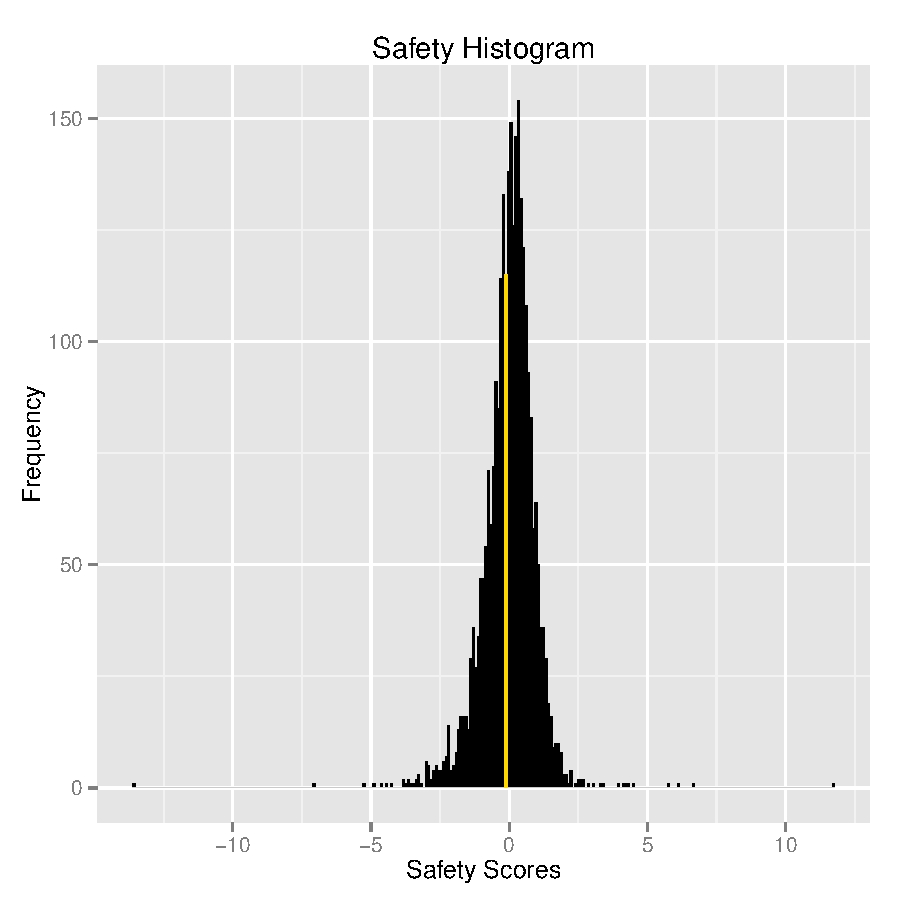
\includegraphics{paper-005}

Functions also exist in order to easily retrieve a specific set of companies.

\begin{Schunk}
\begin{Sinput}
> data(qmjs)
> tickers <- c("GOOG", "IBM", "AAPL")
> selected_qmjs <- get_qmjs(tickers, qmjs)
> summarize(selected_qmjs[[2]])
\end{Sinput}
\begin{Soutput}
Information for:  IBM
_______________________________________
Quality Score:  1.329808
_______________________________________
  profitability      GPOA        ROE       ROA     CFOA       GMAR       ACC
1     0.6367209 0.9048216 0.04271614 0.2893791 0.363422 0.07793538 0.4147032


       growth        GPOA ROE       ROA       CFOA        GMAR        ACC
1 -0.03430372 -0.03446951   0 0.0226805 -0.0122254 -0.05639716 0.01473173


     safety       BAB      IVOL        LEV OhlsonOScore AltmanZScore
1 0.5893127 0.9511291 0.7477697 -0.1908257   -0.1430004    0.3368653


    payouts     EISS      DISS       NPOP
1 0.1380777 0.456594 -0.242883 0.01451857

_______________________________________
\end{Soutput}
\end{Schunk}

\section*{Analyzing the Universe (Of Companies)}
In the quality data set, it can quickly be seen that the growth score for Angies List Inc. is abnormally high, and accounts for virtually all of its quality score. In many cases, it is undesirable to consider companies with high quality scores that are ``driven'' (here defined as composing at least half the quality score) by a single component score. \textbf{qmj} provides a filter.

\begin{Schunk}
\begin{Sinput}
> data(quality)
> head(quality)
\end{Sinput}
\begin{Soutput}
                     name ticker profitability      growth      safety
1         ANGIES LIST INC   ANGI    -0.1575365 24.55764246 -0.89076389
2 SEACOAST BANKING CORP F   SBCF    -0.9552288 21.17749195  0.23623565
3                  AMERCO   UHAL    -0.3350943 19.25596295 -0.16064717
4   GUIDANCE SOFTWARE INC   GUID     0.2245725 13.61798234  0.09569998
5       BROWN & BROWN INC    BRO     0.1484205 -0.04063592 11.76587071
6 CAPITOL FEDERAL FINL IN   CFFN     5.7540587 -0.04904148  5.73770806
     payouts  quality
1 -1.8699982 21.63934
2 -1.0820805 19.37642
3 -1.9855567 16.77466
4 -1.5591484 12.37911
5  0.2254432 12.09910
6  0.2292110 11.67194
\end{Soutput}
\begin{Sinput}
> sans_growth <- filter_companies(quality, filter="growth")
> head(sans_growth)
\end{Sinput}
\begin{Soutput}
                      name ticker profitability      growth     safety
5        BROWN & BROWN INC    BRO     0.1484205 -0.04063592 11.7658707
6  CAPITOL FEDERAL FINL IN   CFFN     5.7540587 -0.04904148  5.7377081
8      CENTURY ALUMINUM CO   CENX    -0.1912805  3.43982232  6.1767505
9  CORRECTIONS CORP OF AME    CXW    -0.3283571  3.22020489  4.1009744
10    ROUSE PROPERTIES INC    RSE     3.6209141  0.04701919  1.8876675
11       PATTERSON COS INC   PDCO    -0.7411908 -0.05296278  0.1659304
      payouts   quality
5   0.2254432 12.099098
6   0.2292110 11.671936
8  -0.1956603  9.229632
9   0.1910389  7.183861
10  0.9855644  6.541165
11  6.7805708  6.152348
\end{Soutput}
\end{Schunk}

If desirable, we may also select specifically for those companies which are driven by a particular component. Note that \textit{remove} is, by default, set to TRUE, and \textit{isolate}, is set to FALSE.

\begin{Schunk}
\begin{Sinput}
> driven_by_profit <- filter_companies(quality, filter="profitability", remove=FALSE, isolate=TRUE)
> head(driven_by_profit)
\end{Sinput}
\begin{Soutput}
                      name ticker profitability      growth     safety
10    ROUSE PROPERTIES INC    RSE      3.620914  0.04701919  1.8876675
14           MARINEMAX INC    HZO      2.705818 -0.01095467  1.1415603
25    TRW AUTOMOTIVE HLDGS    TRW      2.618192 -0.03051664  1.5530658
26          TESLA MTRS INC   TSLA      4.609760 -0.03092323 -0.5101186
27 SBA COMMUNICATIONS CORP   SBAC      2.312696 -0.02110655  1.7126875
31        BANCORPSOUTH INC    BXS      3.183034 -0.11750128  0.7686165
     payouts  quality
10 0.9855644 6.541165
14 1.5434407 5.379865
25 0.1615215 4.302262
26 0.1859741 4.254693
27 0.1624351 4.166712
31 0.1812339 4.015383
\end{Soutput}
\end{Schunk}

Or, we can select for all companies which are not driven by any component score.

\begin{Schunk}
\begin{Sinput}
> well_rounded <- filter_companies(quality, filter="all")
> head(well_rounded)
\end{Sinput}
\begin{Soutput}
                      name ticker profitability      growth    safety   payouts
6  CAPITOL FEDERAL FINL IN   CFFN     5.7540587 -0.04904148 5.7377081 0.2292110
21 HANNON ARMSTRONG SUSTAI   HASI     1.2166640 -0.02772366 1.7356800 1.7275803
22  ADAMAS PHARMACEUTICALS   ADMS     1.6916207  0.50007697 2.2264045 0.2107355
24   OPLINK COMMUNICATIONS   OPLK     0.9992939  1.89816751 1.2105671 0.2178525
33              WATSCO INC    WSO     1.9397013 -0.01815565 1.8758314 0.1712876
34          P C CONNECTION   PCCC     1.4991871 -0.01996304 0.5011669 1.9790272
     quality
6  11.671936
21  4.652201
22  4.628838
24  4.325881
33  3.968665
34  3.959418
\end{Soutput}
\end{Schunk}

It may also be desirable to look at quality scores specific to a subset of our extant universe. For example, it may be desirable to focus on a specific industry, instead of the entire market.

\begin{Schunk}
\begin{Sinput}
> data(companies)
> data(financials)
> data(prices)
> subset_companies <- companies[1:35,]
> subset_qualities <- market_data(subset_companies, financials, prices)
> head(subset_qualities)
\end{Sinput}
\begin{Soutput}
                  name ticker profitability     growth     safety    payouts
1  ACADIA REALTY TRUST    AKR     0.4454608  1.9089319  1.5526137 1.31478094
2  ABBOTT LABORATORIES    ABT     1.7678451 -0.1095279  1.7803241 0.05153694
3 ACADIA HEALTHCARE CO   ACHC     1.1669597  0.5217762  0.3551660 1.00840842
4      1ST SOURCE CORP   SRCE     0.4229837  0.1556518  1.5151657 0.77935661
5 ACACIA RESEARCH CORP   ACTG    -0.1253302  0.3120711 -0.5093214 2.97055627
6               2U INC   TWOU     0.7175041  0.7028707  0.6442629 0.01594466
   quality
1 5.221787
2 3.490178
3 3.052310
4 2.873158
5 2.647976
6 2.080582
\end{Soutput}
\end{Schunk}

\section*{Conclusion}

In the \textbf{qmj} package, we automate AQR's method of assigning quality scores for publicly traded companies in today's market. The package itself provides convenient datasets and utility functions, and it also takes advantage of R's robust nature to allow seamless interaction with functions in the base R package and other packages.
\\
\\
\emph{Ryan Kwon}
\\
\emph{Williams College}
\\
\emph{Williamstown, MA}
\\
\emph{USA}
\\
rhk1@williams.edu
\\
\\
\emph{Anthoney Tsou}
\\
\emph{Williams College}
\\
\emph{Williamstown, MA}
\\
\emph{USA}
\\
at6@williams.edu

\section*{Bibliography}
Asness, Clifford S., Andrea Frazzini, and Lasse H. Pedersen. ``Quality Minus Junk." AQR (2013)
\section*{Appendix}
We calculate quality scores for publicly traded companies in the Russell 3000 Index by summing the z-scores for each company's profitability, growth, safety, and payouts. We attempt to perform the same calculations as AQR does, but we have a few adjustments given the availability of data from public sources. 
\subsection*{Profitability}
Profitability is composed of six variables: gross profits over assets ($GPOA$), return on equity ($ROE$), return on assets ($ROA$), cash flow over assets ($CFOA$), gross margin ($GMAR$), and accruals ($ACC$). $GPOA$ is calculated as gross profits ($GPROF$) over total assets ($TA$). $$GPOA \ = \ \frac{GPROF}{TA}$$ $ROE$ is calculated as net income ($NI$) over book equity ($BE$), which is shareholders' equity (the difference of Total Liabilities and Shareholders' Equity ($TLSE$) with Total Liabilities ($TL$)) - preferred stock (the sum of redeemable preferred stock ($RPS$) and non redeemable preferred stock ($NRPS$)). $$ROE \ = \ \frac{NI}{BE}$$ $ROA$ is calculated as $NI$ over $TA$. $$ROA \ = \ \frac{NI}{TA}$$ $CFOA$ is calculated as $NI$ + depreciation ($DP.DPL$) - changes in working capital ($CWC$) - capital expenditures ($CX$) all over $TA$. $$CFOA \ = \ \frac{NI \ + \ DP.DPL \ - \ CWC \ - \ CX}{TA}$$ $GMAR$ is calculated as $GPROF$ over total revenue ($TREV$). $$GMAR \ = \ \frac{GPROF}{TREV}$$ Finally, $ACC$ is calculated as $DP.DPL$ - $CWC$ all over $TA$. $$ACC \ = \ \frac{DP.DPL \ - \ CWC}{TA}$$ We then standardize all components of profitability to z-scores and then standardize all profitability scores into z-scores. $$Profitability \ = \ z(z_{gpoa} \ + \ z_{roe} \ + \ z_{roa} \ + \ z_{cfoa} \ + \ z_{gmar} \ + \ z_{acc})$$
\subsection*{Growth}
Growth is measured by differences in profitability across a time span of four years. Though AQR recommends measuring growth across a time span of five years, public information that is both consistent and well-organized in 10-K forms is only available for a time span of four years, and it is still too early in the most recent year (2015) for most companies to have submitted a 10-K form. Thus, we measure growth using a time span of four years, which we will update once this year's 10-K form is submitted for each company in the Russell 3000 Index. As of now, $$Growth \ = \ z(z_{\Delta gpoa_{t,t-4}} \ + \ z_{\Delta roe_{t,t-4}} \ + \ z_{\Delta roa_{t,t-4}} \ + \ z_{\Delta cfoa_{t,t-4}} \ + \ z_{\Delta gmar_{t,t-4}} \ + \ z_{\Delta acc_{t,t-4}})$$
\subsection*{Safety}
Safety is composed of six variables: beta ($BAB$), idiosyncratic volatility ($IVOL$), leverage ($LEV$), Ohlson's O ($O$), Altman's Z ($Z$), and earnings volatility ($EVOL$). $BAB$ is calculated as the negative covariance of each company's daily price returns ($pret_{c_i}$) relative to the benchmark daily market price returns ($pret_{mkt}$), in this case the S\&P 500, over the variance of $pret_{mkt}$. $$BAB \ = \ \frac{-cov(pret_{c_i},pret_{mkt})}{var(pret_{mkt})}$$ $IVOL$ is the standard deviation of daily beta-adjusted excess returns. In other words, $IVOL$ is found by running a regression on each company's price returns and the benchmark, then taking the standard deviation of the residuals. Leverage is -(total debt ($TD$) over $TA$). $$Leverage \ = \ -\frac{TD}{TA}$$ 
\\
$$ O \ = \ -(-1.32 \ - \ 0.407 \ * \ log\left(\frac{ADJASSET}{CPI}\right) \ + \ 6.03 \ * \ TLTA \ - \ 1.43 \ * \ WCTA$$
$$ + \ 0.076 \ * \ CLCA \ - \ 1.72 \ * \ OENEG \ - \ 2.37 \ * \ NITA \ - \ 1.83 \ * \ FUTL$$
$$ + \ 0.285 \ * \ INTWO \ - \ 0.521 \ * \ CHIN)$$ 
$ADJASSET$ is adjusted total assets, which is $TA$ + 0.1 * (market equity ($ME$, calculated as average price per share for the most recent year * total number of shares outstanding ($TCSO$) - $BE$)). $$ADJASSET \ = \ TA \ + \ 0.1 \ * \ (ME \ - \ BE)$$ $CPI$, the consumer price index, is assumed to be 100, since we only care about the most recent year. $TLTA$ is book value of debt ($BD$, calculated as $TD$ - minority interest ($MI$) - ($RPS$ + $NRPS$)) over $ADJASSET$. $$TLTA \ = \ \frac{BD}{ADJASSET}$$ $WCTA$ is current assets ($TCA$) - current liabilities ($TCL$) over $TA$. $$WCTA \ = \ \frac{TCA - TCL}{TA}$$ $CLCA$ is $TCL$ over $TCA$. $$ CLCA \ = \ \frac{TCL}{TCA}$$ $OENEG$ is a dummy variable that is 1 if total liabilities ($TL$) is greater than $TA$. $$ OENEG \ = \ TL > TA $$ $NITA$ is $NI$ over $TA$. $$NITA \ = \ \frac{NI}{TA}$$ $FUTL$ is income before taxes ($IBT$) over $TL$. $$FUTL \ = \ \frac{IBT}{TL}$$ $INTWO$ is another dummy variable that is 1 if $NI$ for the current year and $NI$ for the previous year are both negative. $$INTWO \ = \ MAX(NI_t,NI_{t-1}) < 0$$ $CHIN$ is $NI$ for the current year - $NI$ for the previous year all over the sum of the absolute value of $NI$ for the current year and the absolute value of $NI$ for the previous year $$CHIN \ = \ \frac{NI_t \ - \ NI_{t-1}}{|NI_t| + |NI_{t-1}|}$$ Altman's Z is calculated using weighted averages of working capital ($WC$, calculated as $TCA$ - $TCL$), $$WC \ = \ TCA \ - \ TCL$$ retained earnings ($RE$, calculated as $NI$ - dividends per share ($DIVC$) * $TCSO$), $$RE \ = \ NI \ - \ DIVC \ * \ TCSO$$ earnings before interest and taxes ($EBIT$, calculated as $NI$ - Discontinued Operations($DO$) + ($IBT$ - income after tax ($IAT$)) + interest expense ($NINT$)), $$ EBIT \ = \ NI \ - \ DO \ + \ (IBT \ - \ IAT) \ + \ NINT $$ $ME$, and $TREV$, all over $TA$. $$Z \ = \frac{\ 1.2 \ * \ WC \ + \ 1.4 \ * \ RE \ + \ 3.3 \ * \ EBIT \ + \ 0.6 \ * \ ME \ + TREV}{TA}$$ $EBIT$ is likely an overestimate for a given company due to potentially missing information. $EVOL$ is calculated as the standard deviation of $ROE$ for a four year span. AQR recommends the past five years, but for the same reason stated in the Growth section, we use a four year span. $$EVOL = \sigma\left(\sum_{i=t-4}^{t}ROE_i\right)$$ Likewise, we standardize each variable and then standardize each safety measure, so $$Safety \ = \ z(z_{bab} \ + \ z_{ivol} \ + \ z_{lev} \ + \ z_{o} \ + \ z_{z} \ + \ z_{evol})$$ 
\subsection*{Payouts}
Payouts is composed of three variables: net equity issuance ($EISS$), net debt issuance ($DISS$), and total net payout over profits ($NPOP$). $EISS$ is calculated as the negative log of the ratio of $TCSO$ of the most recent year and $TCSO$ of the previous year. $$EISS \ = \ -log\left(\frac{TCSO_t}{TCSO_{t-1}}\right)$$ Though AQR uses split-adjusted number of shares, we are currently using $TCSO$ given available information and will adjust for splits in future iterations of qmj. $DISS$ is calculated as the negative log of the ratio of $TD$ of the most recent year and $TD$ of the previous year. $$DISS \ = \ -log\left(\frac{TD_t}{TD_{t-1}}\right)$$ $NPOP$ is calculated as $NI$ - $\Delta BE$ over a four year span all over sum of $GPROF$ for the past four years (for the same reason as explained in the Growth section). $$NPOP \ = \ \frac{NI - \Delta BE}{\sum_{i=t-4}^{t}GPROF_i}$$
\end{document}
